% ===========================================
% Template for ICMC 2021 in Santiago, Chile (version1)
% adapted from earlier LaTeX paper templates for the ICMC, SMC, etc...
% by Rodrigo F. Cádiz rcadiz@uc.cl
% ===========================================

\documentclass{article}
\usepackage{icmc2021template}
\usepackage{times}
\usepackage{ifpdf}
\usepackage{soul}
\usepackage[english]{babel}
\usepackage{enumitem}
\usepackage{musicography}
\usepackage{amsmath}
\usepackage{arydshln}
\usepackage{amssymb}
\usepackage{caption}
\captionsetup{skip=5pt}
\usepackage{graphics}
 \usepackage{musicography}
%\usepackage{cite}


\usepackage{calc}
\newlength{\maxcollen}

\newcommand{\setmeter}[2]{\ensuremath{%
  \vcenter{\offinterlineskip
    \halign{\hfil##\hfil\cr
            $\scriptstyle#1$\cr
            \noalign{\vskip1pt}
            $\scriptstyle#2$\cr}
  }}%
}

%%%%%%%%%%%%%%%%%%%%%%%% Some useful packages %%%%%%%%%%%%%%%%%%%%%%%%%%%%%%%
%%%%%%%%%%%%%%%%%%%%%%%% See related documentation %%%%%%%%%%%%%%%%%%%%%%%%%%
%\usepackage{amsmath} % popular packages from Am. Math. Soc. Please use the 
%\usepackage{amssymb} % related math environments (split, subequation, cases,
%\usepackage{amsfonts}% multline, etc.)
%\usepackage{bm}      % Bold Math package, defines the command \bf{}
%\usepackage{paralist}% extended list environments
%%subfig.sty is the modern replacement for subfigure.sty. However, subfig.sty 
%%requires and automatically loads caption.sty which overrides class handling 
%%of captions. To prevent this problem, preload caption.sty with caption=false 
%\usepackage[caption=false]{caption}
%\usepackage[font=footnotesize]{subfig}

% ====================================================
% ================ Define title and author names here ===============
% ====================================================
%user defined variables
\def\papertitle{MusAssist: A Domain Specific Language for Music Notation}
\def\firstauthor{Ilana Shapiro}
\def\secondauthor{Second Author}
\def\thirdauthor{Third Author}
\def\fourthauthor{Fourth Author}
\def\fifthauthor{Fifth Author}
\def\sixthauthor{Sixth Author}

% adds the automatic
% Saves a lot of output space in PDF... after conversion with the distiller
% Delete if you cannot get PS fonts working on your system.

% pdf-tex settings: detect automatically if run by latex or pdflatex
\newif\ifpdf
\ifx\pdfoutput\relax
\else
   \ifcase\pdfoutput
      \pdffalse
   \else
      \pdftrue
  \fi
\fi

\ifpdf % compiling with pdflatex
  \usepackage[pdftex,
    pdftitle={\papertitle},
    pdfauthor={\firstauthor, \secondauthor, \thirdauthor},
    bookmarksnumbered, % use section numbers with bookmarks
    pdfstartview=XYZ % start with zoom=100% instead of full screen; 
                     % especially useful if working with a big screen :-)
   ]{hyperref}
  %\pdfcompresslevel=9

  \usepackage[pdftex]{graphicx}
  % declare the path(s) where your graphic files are and their extensions so 
  %you won't have to specify these with every instance of \includegraphics
  \graphicspath{{./figures/}}
  \DeclareGraphicsExtensions{.pdf,.jpeg,.png}

  \usepackage[figure,table]{hypcap}

\else % compiling with latex
  \usepackage[dvips,
    bookmarksnumbered, % use section numbers with bookmarks
    pdfstartview=XYZ % start with zoom=100% instead of full screen
  ]{hyperref}  % hyperrefs are active in the pdf file after conversion

  \usepackage[dvips]{epsfig,graphicx}
  % declare the path(s) where your graphic files are and their extensions so 
  %you won't have to specify these with every instance of \includegraphics
  \graphicspath{{./figures/}}
  \DeclareGraphicsExtensions{.eps}

  \usepackage[figure,table]{hypcap}
\fi

%setup the hyperref package - make the links black without a surrounding frame
\hypersetup{
    colorlinks,%
    citecolor=black,%
    filecolor=black,%
    linkcolor=black,%
    urlcolor=black
}


% ====================================================
% ================ Title and author info starts here ===============
% ====================================================
% Title.
% ------
\title{\papertitle}

% Authors
% Please note that submissions are anonymous, therefore 
% authors' names should not be VISIBLE in your paper submission.
% They should only be included in the camera-ready version of accepted papers.
% uncomment and use the appropriate section (1, 2 or 3 authors)
%
% Single address
% To use with only one author or several with the same address
% ---------------
%\oneauthor
%   {\firstauthor} {Affiliation \\ %
%     {\tt \href{mailto:author@uc.cl}{author@uc.cl}}}

%Two addresses
% the default spacing is 1.5in, but this can be reduced to 0.5in or less, if needed
%--------------
% \twoauthors
%   {1.5in}
%   {\firstauthor} {Affiliation1 \\  %
%     {\tt \href{mailto:author1@uc.cl}{author1@uc.cl}}}
%   {\secondauthor} {Affiliation2 \\  %
%     {\tt \href{mailto:author2@uc.cl}{author2@uc.cl}}}

% Three addresses
% the default spacing is 0.5in, but this can be reduced to 0.3in or less, if needed
% --------------
 \oneauthor
  %  {0.5in}
   {\firstauthor} {Pomona College \\ %
     {\tt \href{mailto:issa2018@mymail.pomona.edu}{issa2018@mymail.pomona.edu}}}
  %  {\secondauthor} {Affiliation2 \\ %
  %    {\tt \href{mailto:author2@myorg.org}{author2@myorg.org}}}
  %  {\thirdauthor} { Affiliation3 \\ %
  %    {\tt \href{mailto:author3@myorg.org}{author3@myorg.org}}}

% Four addresses
% the default spacing is 1.5in, but this can be reduced to 0.5in or less, if needed
% --------------
% \fourauthors
%   {1.5in}
%   {\firstauthor} {Affiliation1 \\ %
%     {\tt \href{mailto:author1@uc.cl}{author1@uc.cl}}}
%   {\secondauthor} {Affiliation2 \\ %
%     {\tt \href{mailto:author2@uc.cl}{author2@uc.cl}}}
%   {\thirdauthor} { Affiliation3 \\ %
%     {\tt \href{mailto:author3@uc.cl}{author3@uc.cl}}}
%   {\fourthauthor} { Affiliation4 \\ %
%     {\tt \href{mailto:author4@uc.cl}{author4@uc.cl}}}

% Five addresses
% the default spacing is 0.5in, but this can be reduced to 0.3in or less, if needed
% --------------
% \fiveauthors
%   {0.5in}
%   {\firstauthor} {Affiliation1 \\ %
%     {\tt \href{mailto:author1@uc.cl}{author1@uc.cl}}}
%   {\secondauthor} {Affiliation2 \\ %
%     {\tt \href{mailto:author2@uc.cl}{author2@uc.cl}}}
%   {\thirdauthor} { Affiliation3 \\ %
%     {\tt \href{mailto:author3@uc.cl}{author3@uc.cl}}}
%   {\fourthauthor} { Affiliation4 \\ %
%     {\tt \href{mailto:author4@uc.cl}{author4@uc.cl}}}
%   {\fifthauthor} { Affiliation5 \\ %
%     {\tt \href{mailto:author5@uc.cl}{author5@uc.cl}}}

% Six addresses
% the default spacing is 0.5in, but this can be reduced to 0.3in or less, if needed
% --------------
% \sixauthors
%   {0.5in}
%   {\firstauthor} {Affiliation1 \\ %
%     {\tt \href{mailto:author1@uc.cl}{author1@uc.cl}}}
%   {\secondauthor} {Affiliation2 \\ %
%     {\tt \href{mailto:author2@uc.cl}{author2@uc.cl}}}
%   {\thirdauthor} { Affiliation3 \\ %
%     {\tt \href{mailto:author3@uc.cl}{author3@uc.cl}}}
%   {\fourthauthor} { Affiliation4 \\ %
%     {\tt \href{mailto:author4@uc.cl}{author4@uc.cl}}}
%   {\fifthauthor} { Affiliation5 \\ %
%     {\tt \href{mailto:author5@uc.cl}{author5@uc.cl}}}
%   {\sixthauthor} { Affiliation6 \\ %
%     {\tt \href{mailto:author6@uc.cl}{author6@uc.cl}}}


% ====================================================
% =============== The document content starts here ===============
% ====================================================
\begin{document}
%
\capstartfalse
\maketitle
\capstarttrue
%
\begin{abstract}
MusAssist is an external, declarative domain specific language for music notation that bridges the abstraction gap between music theory and composition. Users can describe complex musical 
templates for all triads and seventh chords, 
all diatonic as well as chromatic and whole tone scales, the five primary cadences (including imperfect authentic), 
and the four primary harmonic sequences with desired length. Uniquely, the level of abstraction of a template 
MusAssist matches that of the theoretical musical structure it describes (e.g. users can specify
 a harmonic sequence without manually lowering the granularity to chords and notes). Thus, users can write out specifications precisely at the conceptual levels of the musical theoretical structures 
 they would organically conceive when composing by hand. In MusAssist, users can also change key signatures, 
 start a new measure, and describe fundamental musical objects such as notes, rests, and chords comprised of 
 custom collections of notes. A musical expression described by a higher level template is expanded  
 (i.e. the level of abstraction is fully lowered to notes) by the 
 Haskell-based MusAssist compiler and translated to MusicXML, a language accepted by most 
 major music notation softwares, for further manual editing. 
\end{abstract}


\section{Introduction}\label{sec:introduction}
When writing music, composers must manually transition from musical theoretical concepts to notes on a page.
This process can be tedious and slow, requiring the composer to expand by hand complex structures, such as cadences and sequences,
to the notes they constitute. The level of abstraction of the musical theoretical structure is 
higher than what the composer actually writes. 

Domain specific languages, or DSLs, 
are programming languages highly specialized for a specific application and thus characterized by limited expressiveness.
An \textit{external DSL} has custom syntax that is separated from the primary language of its application. 

This paper presents MusAssist, an external, declarative DSL for music notation that bridges the divide between
music theory and notation. Users describe a composition in MusAssist's straightforward, high-level syntax, modeled
around the musical elements composers organically conceive when notating by hand, and the MusAssist compiler automates the expansion of these elements to their constituent notes. MusAssist's declarative programming paradigm was chosen to further correspond with the declarative nature of handwritten music. 

Fundamentally, MusAssist supports notes (including rests) and custom chords (i.e. any desired collection of notes)
in the octave and key of choice, as well as commands to change the key signature or start a new measure.
 MusAssist is unique in that users can also write specifications for complex musical templates \textit{at the same level of abstraction
as the musical theoretical structures they describe}. MusAssist supports templates for
\textbf{chords} and \textbf{arpeggios} (all triads and seventh chords in any inversion),
\textbf{scales} (major, natural/harmonic/melodic minor, chromatic, and whole tone),
\textbf{cadences} (perfect authentic, imperfect authentic, plagal, half, deceptive), and 
\textbf{harmonic sequences} (ascending
fifths, descending fifths, ascending 5-6, descending 5-6) of a desired length. The musical expression 
described by a specification is expanded (i.e. the abstraction level is
fully lowered to notes) by the Haskell-based MusAssist compiler.

The target language of the MusAssist compiler is MusicXML, itself a DSL that is an extension of
XML (Extensible Markup Language). MusicXML is accepted by most major notation software programs (such as MuseScore). 
Thus, users can open can open the resulting MusicXML file of a compiled MusAssist composition in MuseScore or another
program for further customization and editing, bypassing the need to write out complex musical templates by hand at a 
note or chord granularity. Beyond a professional music compositional aid, MusAssist may be particularly 
helpful to music theory students as an educational tool, enabling them to visualize the relationship between a theoretical musical structure 
and its expanded form, such as a cadence and the chords resulting from its expansion.

The paper is organized as follows. Section \ref{sec:related_work} begins by presenting related work in music notation DSLs. Section \ref{sec:language_features} then outlines features of the MusAssist languages, followed by a concrete example in Section \ref{sec:sample_program}. Section \ref{sec:compiler_structure} outlines the MusAssist compiler structure, and Section \ref{sec:template_expansions} summarizes the central logic behind MusAssist's formalization of musical theoretical structures. Finally, conclusions are future work are discussed.

%-----------------------------------------------------------------------------------------------------------------------------------------------------

\section{Related Work}\label{sec:related_work}

The era of music DSLs began in 2008 with Ge Wang's ChucK audio processing language, which  
spans the application domains of ``methods for sound synthesis, physical modeling of real-time world artifacts and spaces (e.g., 
musical instruments, environmental sounds), analysis and information retrieval of sound and music, to 
mapping and crafting of new controllers and interfaces (both software and physical) for music, 
algorithmic/generative processes for automated or semi-automatic composition and accompaniment, [and] 
real-time music performance." \cite{wang_2008}. 
Since then, researchers have taken advantage of the increased flexibility afforded to DSLs via their limited expressiveness to create
music DSLs tailored towards notation, algorithmic composition, signal processing, live coding with music performance, and more. In the 
 notation domain, MusicXML, LilyPond, and PyTabs stand out.

Michael Good's MusicXML is an Internet-friendly, XML-based, declarative DSL capable of representing Western music 
notation and sheet music since c. 1600. 
It acts as an ``interchange format for applications in music notation, music analysis, music information retrieval, 
and musical performance," thus supporting sharing between specialized applications. \cite{good_2013}

MusicXML attempts to emulate for online sheet music and music software what the popular MIDI format 
did for electronic instruments. It is derived from XML in order to help solve the music 
interchange problem: to create a standardized method to represent complex, structured data in order to support 
smooth interchange between ``musical notation, performance, analysis, and retrieval applications." XML has the 
desired qualities of ``straightforward usability over the Internet, ease of creating documents, and human readability" 
that translate directly into the musical domain, and it is more powerful and expressive 
than MIDI. \cite{good_2001}

MusicXML is more expressive than MusAssist, but the abstraction level of all musical elements is extremely low (i.e. chords must be written out 
as individual notes) and its syntax is cumbersome and tedious to write by hand. However, its expressiveness makes MusicXML an excellent target compilation language for MusAssist's user-friendly syntax and high-level musical theoretical templates.

LilyPond, an external declarative DSL created by Han-Wen Nienhuys and 
Jan Nieuwenhuizen, is similar to MusAssist. It features a ``modular, extensible and programmable 
compiler" written in Scheme to generate Western music notation of excellent quality and supports the mixing of text and music elements. 
Text-based \textit{musical expressions}, or fragments of music with 
set durations, are compiled to an aesthetically formatted score.\cite{nienhuys_nieuwenhuizen_2003}

LilyPond and MusAssist are both music notation DSLs tailored to non-programming audiences. However, 
they differ in two fundamental areas: 
(1) MusAssist supports complex music templates at the levels of abstraction of the 
musical structures they represent, whereas LilyPond only supports 
more granular, low level composition of individual notes and chords, and (2) the output of the MusAssist compiler is intentionally editable via
notation software, unlike LilyPond's compiler, which produces a static, printable PostScript or PDF file by 
taking in a file with a formal representation of the desired music.
\cite{nienhuys_nieuwenhuizen_2003}

Simic et al.'s external, declarative DSL PyTabs similarly is geared toward music notation, but in a different
domain than MusAssist. Specifically, 
the authors attempt to solve visual problem of  tablature  notation, 
and the lack of standardization of how  to specify note duration in this format, by consolidating 
these issues into a formal language. Tablature notation is outside the scope of MusAssist's focus on Western 
musical theoretical structures.
 \cite{simic_bal_dejanovic_vaderna}.

%-----------------------------------------------------------------------------------------------------------------------------------------------------

\section{Language Features}\label{sec:language_features}
\subsection{Low-Level Fundamentals}
On the most basic level, MusAssist supports individual rests and notes. Rests are  
given a duration from sixteenth to whole note, and notes are further defined by note name (A to G), 
accidental (double flat to double sharp), and octave (1 to 8, after the range of a piano).
Just as in normal notation, the absence of an accidental indicates natural quality.
Finally, users can also define ``custom chords,'' or user-defined lists of individual notes.
These are not considered templates as the high-level description of the chord is not given, and the
granularity is at the note level.

\subsection{High-Level Templates}
MusAssist supports templates for chords, arpeggios, scales, cadences, and harmonic sequences, specified uniquely
at the abstraction level of the musical theoretical structures they represent.

Precisely as in music theory, chords are specified by the 
root note (defined as the fundamental MusAssist note is),
quality (major, minor, augmented, diminished, or half diminished), 
inversion (root, first, second, or third), and 
chord type (triad or seventh). 
Half diminished and third inversion options apply to seventh chords only. The root note 
cannot have a double accidental, as this can introduce triple accidentals in the chord, which MusAssist
does not support.

Arpeggios are defined precisely as MusAssist chords are, as arpeggios are simply broken chords.

Similarly, diatonic scales are given by key and scale type (major, and harmonic/melodic/natural minor), while non-diatonic scales are simply specified by their type (chromatic or whole tone). A scale is either ascending or descending, must be given a length, and does not necessarily begin on the tonic -- the start note must be supplied (defined just as the fundamental MusAssist note is). Following convention, chromatic scales are notated with sharps when ascending and flats when descending. 

Cadences are specified by cadence type (perfect or imperfect authentic, half, plagal, 
or deceptive) and key (defined by the fundamental MusAssist note and a quality, either major or minor). 
Currently, MusAssist only supports a single treble clef line. Thus, cadences are written out in the 
upper voices only, in keyboard voice leading style and incorporating principles of smooth voice leading.

Based on the principles of functional harmony, there are several ways to represent a cadence. 
In MusAssist, the following representations were chosen (\tabref{table:cadences}). The major version is presented first, 
with the minor version following in parentheses.
\vspace{-2mm}
\begin{table}[h]
  \begin{center}
    \renewcommand{\arraystretch}{1.5}
\begin{tabular}{|l|l|}
\hline
Perfect Authentic & IV-V-I (iv-V-i) \\ \hline
Imperfect Authentic & IV-vii$^{\text{o}{6 \atop 4}}$-I$^{6 \atop 4}$ (iv-vii$^{\text{o}{6 \atop 4}}$-i$^{6 \atop 4}$) \\ \hline
Plagal & IV$^{6 \atop 4}$-I (iv$^{6 \atop 4}$-I) \\ \hline
Deceptive & IV-V$^{6 \atop 4}$-vi$^{6 \atop 4}$ (iv-V$^{6 \atop 4}$-VI$^{6 \atop 4}$) \\ \hline
Half & IV-ii$^6$-V (iv-ii$^{\text{o}6}$-V) \\ \hline
\end{tabular}
\caption{MusAssist Cadences Summary}\label{table:cadences}
\end{center}
\vspace{-7mm}
\end{table}

All cadences except perfect authentic are built exclusively with triads.
Perfect authentic cadences also double the root in the final chord to simulate the 4-5-1 bass line
as well as to preserve the requisite 2-1 downward step in the uppermost voice. 
This is demonstrated in \figref{fig:perfauth}, produced with the MusAssist syntax

\vspace{1mm}
\noindent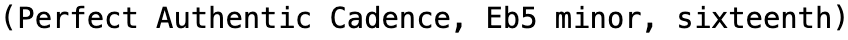
\includegraphics[width=0.45\textwidth]{images/perfauth_code}\\
\vspace{-2mm}
\noindent compiled and loaded into MuseScore notation software.
\vspace{-1mm}
\begin{figure}[h!]
\centering
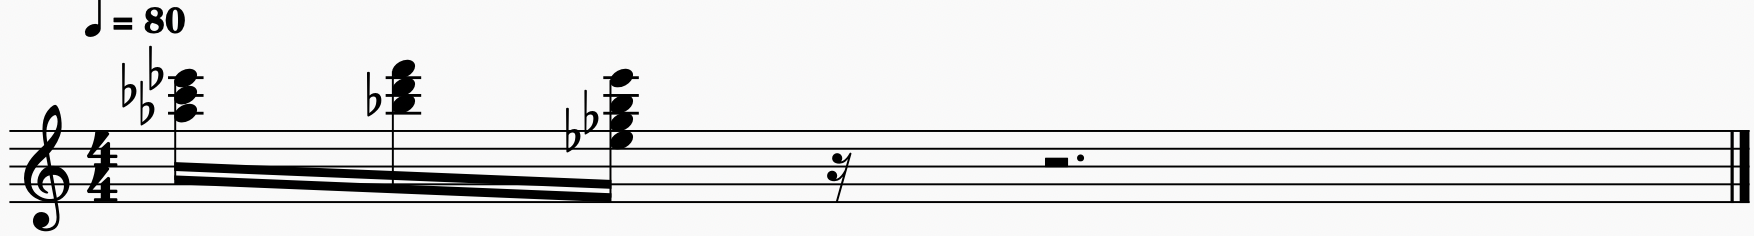
\includegraphics[width=0.45\textwidth]{images/perfauth}
  \caption{Perfect Authentic Cadence in E\musFlat\; minor \label{fig:perfauth}}
  \vspace{-3mm}
\end{figure}

Finally, harmonic sequences are specified by harmonic sequence type (ascending fifths,
descending fifths, ascending 5-6, descending 5-6), key (just as in cadences), duration of each chord,
and length of the sequence. Since MusAssist does not yet support multi-line composition, harmonic sequences are 
written like cadences in keyboard-style voice leading. 

In music theory, harmonic sequences can be implemented in several ways depending on desired inversion scheme. Though the
upper-voice harmonization of a harmonic sequence need not follow the direction in the sequence’s
name, MusAssist chooses a chord inversion and voice leading pattern such that each sequence does
align with the direction of its name (i.e. ascending-named sequences will ascend directionally) 
and also maximizes smooth voice leading. The chosen patterns for each MusAssist sequence are summarized in \tabref{table:harmseq}.
All sequences are shown in major for the sake of example, but their inverse in minor is equally supported. 
Each consists of fourteen distinct chords before repeating in the subsequent octave. 
\vspace{-2mm}
\begin{table}[h!]

  \begin{center}
    \setlength{\maxcollen}{\widthof{vii$^{\text{o}{6 \atop 4}}$}}
    \resizebox{\columnwidth}{!}{
  \begin{tabular}{|c|@{}c@{}|}
  \hline
  Ascending Fifths  & \renewcommand{\arraystretch}{1.5}
                    \begin{tabular}{p{\maxcollen}p{\maxcollen}p{\maxcollen}p{\maxcollen}p{\maxcollen}} 
                        I$^{6 \atop 4}$ & V                & ii$^{6 \atop 4}$            & vi              & iii$^{6 \atop 4}$ \\ \hdashline
                        vii$^\text{o}$  & IV$^{6 \atop 4}$ & I                           & V$^{6 \atop 4}$ & ii                \\ \hdashline
                        vi$^{6 \atop 4}$ & iii             & vii$^{\text{o}{6 \atop 4}}$ & IV              
                    \end{tabular} \\ \hline 
  Descending Fifths & \renewcommand{\arraystretch}{1.5}
                    \begin{tabular}{p{\maxcollen}p{\maxcollen}p{\maxcollen}p{\maxcollen}p{\maxcollen}} 
                      I                & IV$^{6 \atop 4}$ & vii$^\text{o}$  & iii$^{6 \atop 4}$ & vi                          \\ \hdashline
                      ii$^{6 \atop 4}$ & V                & I$^{6 \atop 4}$ & IV                & vii$^{\text{o}{6 \atop 4}}$ \\ \hdashline
                      iii              & vi$^{6 \atop 4}$ & ii              & V$^{6 \atop 4}$
                    \end{tabular} \\ \hline
  Ascending 5-6     & \renewcommand{\arraystretch}{1.5}
                    \begin{tabular}{p{\maxcollen}p{\maxcollen}p{\maxcollen}p{\maxcollen}p{\maxcollen}} 
                      I     & vi$^6$ & ii              & vii$^{\text{o}6}$ & iii      \\ \hdashline
                      I$^6$ & IV     & ii$^6$          & V                 & iii$^6$  \\ \hdashline 
                      vi    & IV$^6$ & vii$^\text{o}$  & V$^6$           
                    \end{tabular} \\ \hline
  Descending 5-6    & \renewcommand{\arraystretch}{1.5}
                    \begin{tabular}{p{\maxcollen}p{\maxcollen}p{\maxcollen}p{\maxcollen}p{\maxcollen}} 
                      I$^{6 \atop 4}$ & V                & vi$^{6 \atop 4}$ & iii                         & IV$^{6 \atop 4}$ \\ \hdashline 
                      I               & ii$^{6 \atop 4}$ & vi               & vii$^{\text{o}{6 \atop 4}}$ & IV               \\ \hdashline 
                      V$^{6 \atop 4}$  & ii               & iii$^{6 \atop 4}$           & vii$^\text{o}$  
                    \end{tabular} \\ \hline
  \end{tabular}
  }
  
\caption{MusAssist Harmonic Sequences Summary}\label{table:harmseq}
\end{center}
\end{table}

\vspace{-8mm}
\subsection{Additional Features}
Beyond compositional elements, users can set the key signature at the beginning
of any measure up to seven sharps or flats by specifying note name, accidental, and quality (sharp or flat).
Users can also start a new measure or create a blank measure. Finally,
users can assign MusAssist expressions to string labels and reuse them later in the program (the labels 
are syntactic sugar for the expressions). MusAssist
comments are designated with \verb!//!.

The tempo for all MusAssist programs
is set at \musQuarter\;= 80bpm and cannot currently be changed.
This also apples to the time signature, which is set at \setmeter{4}{4}.

All compiled MusAssist programs adhere to standard notation conventions. 
Notes and rests are broken over barlines as well as over the strong beat (beat three) of the measure.
They are divided greedily into valid rhythmic units (i.e. from sixteenth to whole note) 
ordered either least to greatest, or greatest to least in the case of spillage over the barline into the following measure.
%-----------------------------------------------------------------------------------------------------------------------------------------------------
\section{Sample Program}\label{sec:sample_program}
The full breadth of MusAssist's syntax is demonstrated in \figref{fig:example_program_code}, and \figref{fig:example_program} is the result of opening the compiled MusicXML code in MuseScore. 

\begin{figure}[h!]
\centering
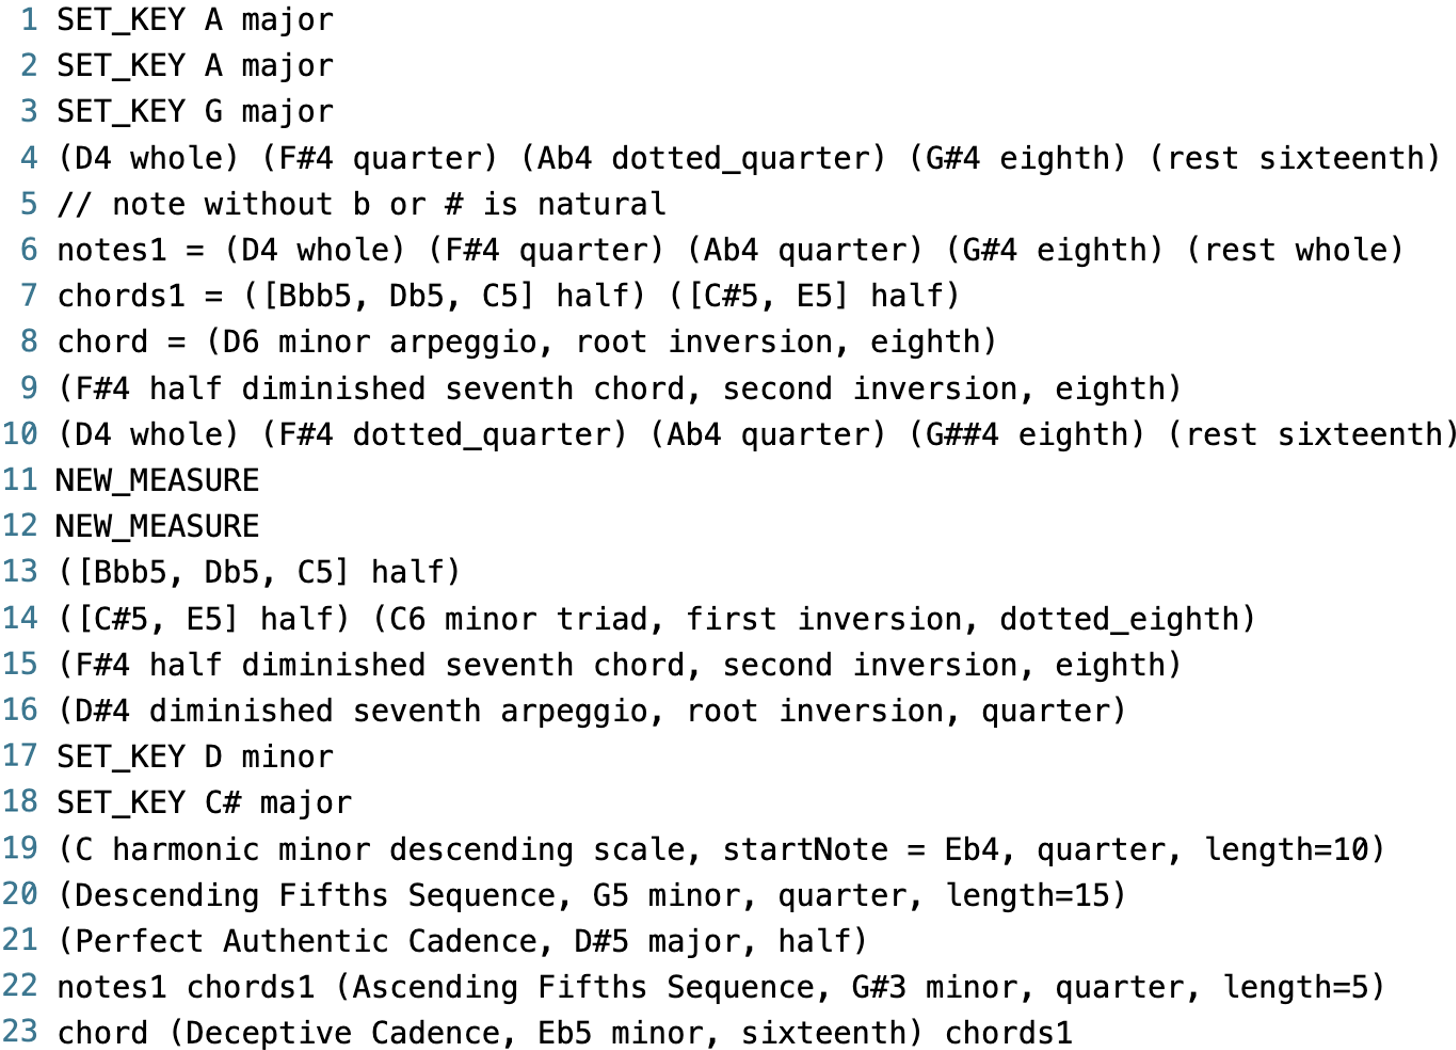
\includegraphics[width=0.5\textwidth]{images/example_program_code}
\vspace{-4mm}
\caption{MusAssist Syntax}\label{fig:example_program_code}
\end{figure}
\vspace{-6mm}
\begin{figure}[h!]
\centering
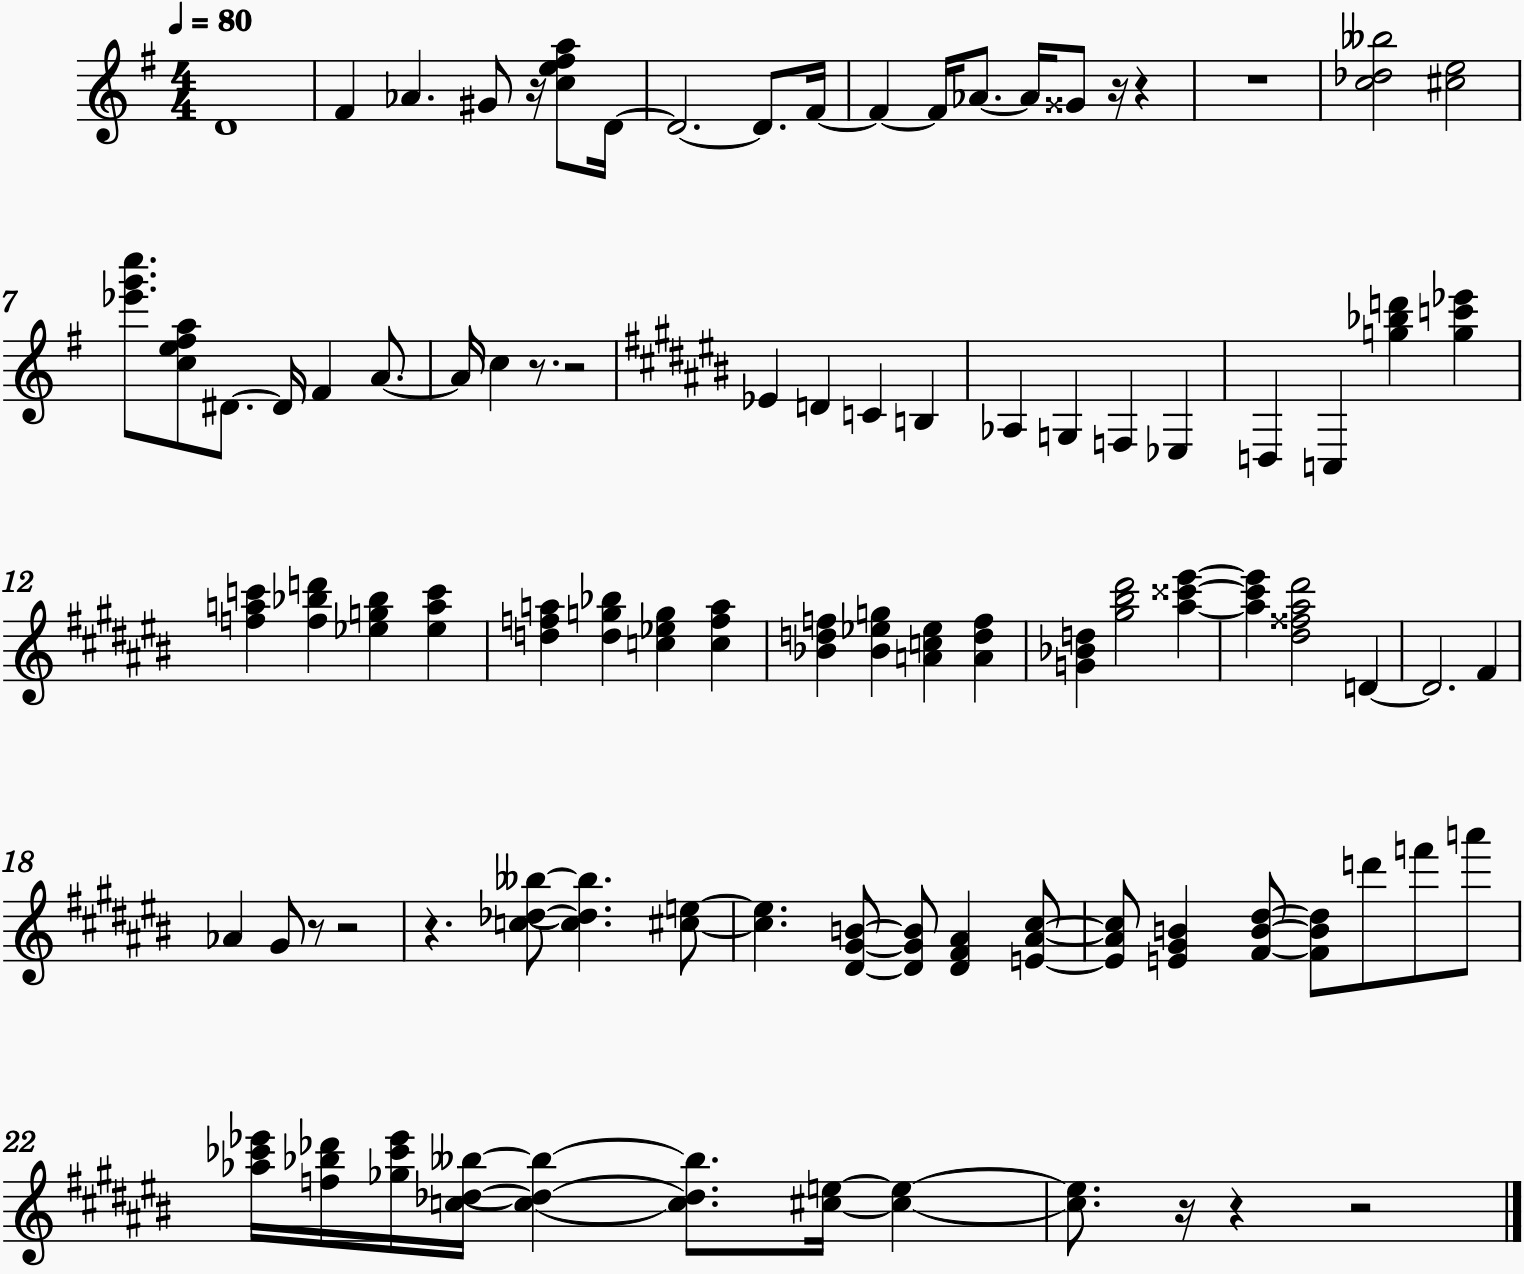
\includegraphics[width=0.5\textwidth]{images/example_program}
\caption{Compiled MusAssist Program in MuseScore}\label{fig:example_program}
\vspace{-3mm}
\end{figure}
  
Notice the following in \figref{fig:example_program_code}:
\vspace{-2mm}
\begin{itemize}
\itemsep0em
\item The key signature can be changed consecutively arbitrarily many times; only the last will take effect (as seen m. 1 and m. 12).
\item Note durations are broken both on the strong beat and on the barline (such as in mm. 2-4). 
\item Labeled phrases are not notated until the label is referenced, rather than defined.
\end{itemize}

%-----------------------------------------------------------------------------------------------------------------------------------------------------

\section{Compiler Structure}\label{sec:compiler_structure}

The MusAssist compiler is written in Haskell. Its high-level structure is as follows: 

\begin{enumerate}
\itemsep0em 
  \item MusAssist concrete syntax is parsed into abstract syntax, represented as 
  Haskell algebraic data types (ADTs). Parser combinators were chosen for their flexibility
  and easy customization. Parsec, an industrial strength parser library, is used, and 
  Parsec’s helper module Token handles lexing. The parse preserves the abstraction 
  level of all templates.

  \item All templates, now represented as ADTs, are expanded using the logic in Section \ref{sec:template_expansions} until the granularity reaches the note level. 
  The result of this intermediate stage is abstract syntax whose abstraction level
  matches that of the target language MusicXML. 

  \item The low-level abstract syntax resulting from the fully expanded templates is 
  translated to MusicXML. This step contains the temporal logic that subdivides notes and rests across
  barlines and strong beats.
\end{enumerate}

The resulting MusicXML file can then be opened in music notation software 
for viewing and further editing. 

%-----------------------------------------------------------------------------------------------------------------------------------------------------

\section{Template Expansion Logic}\label{sec:template_expansions}
MusAssist's most powerful feature is its ability to formalize musical theoretical templates 
to automate their expansion so the user can specify them at the elevated level of abstraction 
of the musical theoretical structures they describe. This section summarizes the logic underlying the expansions.

\subsection{Backbone Logic}
\subsubsection{Generating Notes in a Diatonic Scale}
\label{sec:note_generate}
Most MusAssist templates are built upon the diatonic scale. In order to formalize their expansions, we must first implement logic to generate a note in a diatonic scale of specified quality (major or minor), given a positive interval within one octave of the specified tonic. To generate the note, we need to determine the note name, octave, and accidental.

To determine note name, we simply transverse up the order of note names (ordered as the C major scale is) from the tonic to the target interval. 

The desired octave is either the same as the the tonic's, or one greater than the tonic's if the desired note name comes before the tonic note name in the C major scale. For instance, as seen in \figref{note_octaves}, the red note names D, E, and F come before G in the C major scale, and the octave number of each is one higher than the tonic in a G major scale. 

\vspace{-2mm}
\begin{figure}[h!]
\centering
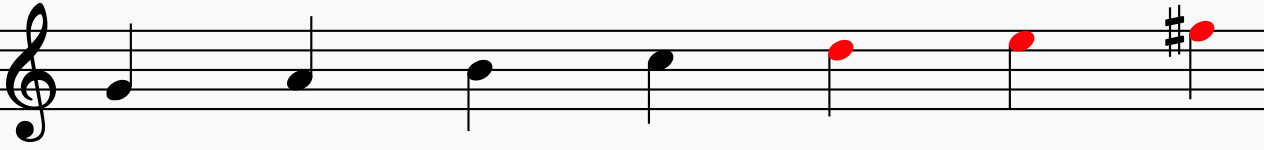
\includegraphics[width=0.3\textwidth]{images/note_octave_logic}
\caption{\centering Octave Analysis of G Major Scale}
\label{note_octaves}
\vspace{-3mm}
\end{figure}

In any key, a perfect interval will have the same accidental as the tonic. To work out the logic behind the accidental of a desired imperfect interval, consider \figref{maj_seconds}. Here, we consider all single-accidental key signature names (even invalid ones that contain double sharps or flats, in order to establish the pattern).  Key signature names are grouped under the accidental of the note that is the desired interval from the tonic. For instance, in the key of A\musFlat\;, the major second interval from the tonic is B\musFlat. The accidental of B\musFlat\; is \musFlat, so A\musFlat\; falls under the \musFlat\; column in \figref{maj_seconds}.
\vspace{-2mm}
\begin{figure}[h!]
\centering
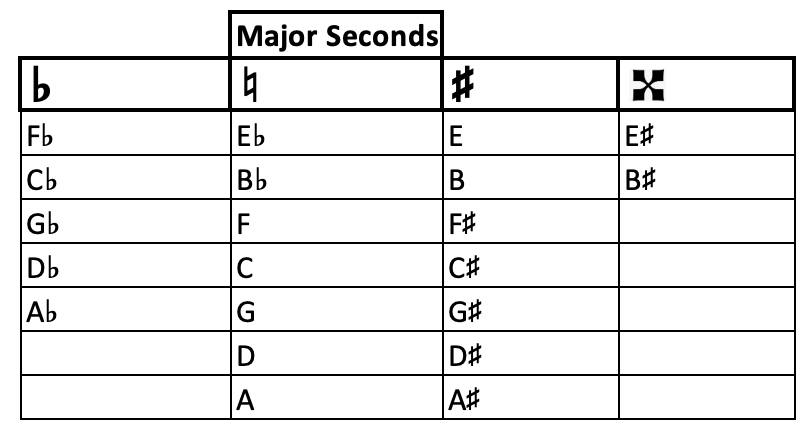
\includegraphics[width=0.3\textwidth]{images/maj_seconds}
\caption{Accidental of Major Second from Tonic per Key}
\label{maj_seconds}
\vspace{-2mm}
\end{figure}

From \figref{maj_seconds} we see that given any key, the major second above the tonic has the same accidental as the tonic, except for the any key with E or B in its name. Here, the accidental is ``lifted"   (i.e. \musFlat $\rightarrow$ \musNatural, \musNatural $\rightarrow$ \musSharp, and \musSharp $\rightarrow$ \musDoubleSharp).

A similar pattern emerges for minor thirds, major sixths, and minor sevenths. Using the result of this analysis, we can determine the accidentals of the inverse qualities (i.e. major $\leftrightarrow$ minor) of the imperfect intervals by either lowering the computed accidental when going from major to minor, or lifting it otherwise.  %We now have all the elements to generate the desired note in the diatonic scale.

\subsubsection{Generating Triads in a Diatonic Scale}
\label{sec:chord_generate}
Generating triads in a diatonic scale becomes relevant for the highest level templates that are conceptualized in music theory with chords rather than notes (namely, cadences and harmonic sequences). Note that these generated triads are still themselves chord templates, albeit at one abstraction level lower than the original musical theoretical structure, and thus require further expansion at a later step. The goal here is simply to automate the generation of chord templates for triads in a diatonic scale given a specified tonic tone and quality (major or minor), inversion, and positive interval within one octave of the tonic for the chordal root. 

In order to complete the chord template definition from the supplied information, we simply need to determine the desired chord quality. Music theory dictates that the major diatonic scale contains the triads I-ii-iii-IV-V-vi-vii$^\text{o}$, and the minor diatonic scale contains the triads i-ii$^\text{o}$-III-iv-v-VI-VII. Using this, we can thus compute the triad quality from the tonic quality and the supplied interval between tonic and desired chordal root.

\subsection{Template Expansions}
\subsubsection{Scales}
The expansion of all major and natural/harmonic/melodic minor scales is derived from the logic in Section \ref{sec:note_generate}. The scale is thus generated in relation to the tonic, rather than the specified start note. The tonic is always set below the start note so that the initial interval between tonic and start note is positive, with the interval then increasing for ascending scales and descending otherwise until the desired scale length is reached. If the tonic is reached in the scale generation, we reset the tonic to be one octave higher or lower (depending on the scale direction), so that the interval between the next note in the scale and the current tonic is always positive and within a single octave. Finally, consider that all minor scales are treated as natural when generating their notes; if needed, the note is modified afterwards in order to appropriately raise the sixth and/or seventh scale degree for harmonic and melodic minor scales.

For the nondiatonic scales (chromatic and whole tone), C is set as the ``tonic" for the purposes of determining the octave. Just like diatonic scales, the tonic octave is shifted appropriately if we pass it during the scale generation.

As seen in \figref{chromatic}, chromatic scales always ``double" the note name, with the directional accidental (sharp for ascending, flat for descending) falling on the second occurrence. There are two exceptions for each direction, marked in red in \figref{chromatic}: E and B are ``single" notes in the ascending version, as are C and F for the descending version.
\vspace{-2mm}
\begin{figure}[h!]
\centering
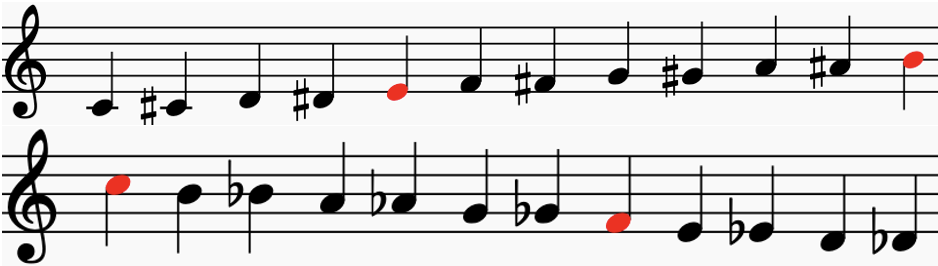
\includegraphics[width=0.4\textwidth]{images/chromatic}
\caption{Chromatic Scales}
\label{chromatic}
\vspace{-3mm}
\end{figure}

If we are in a single note, we simply move up the scale. Otherwise, we repeat it and insert an accidental on the second occurrence.

Whole tone scales form a similar paradigm. As seen in \figref{chromatic}, the ascending whole tone scale is missing the note B, while the descending is missing C. 
\vspace{-2mm}
\begin{figure}[h!]
\centering
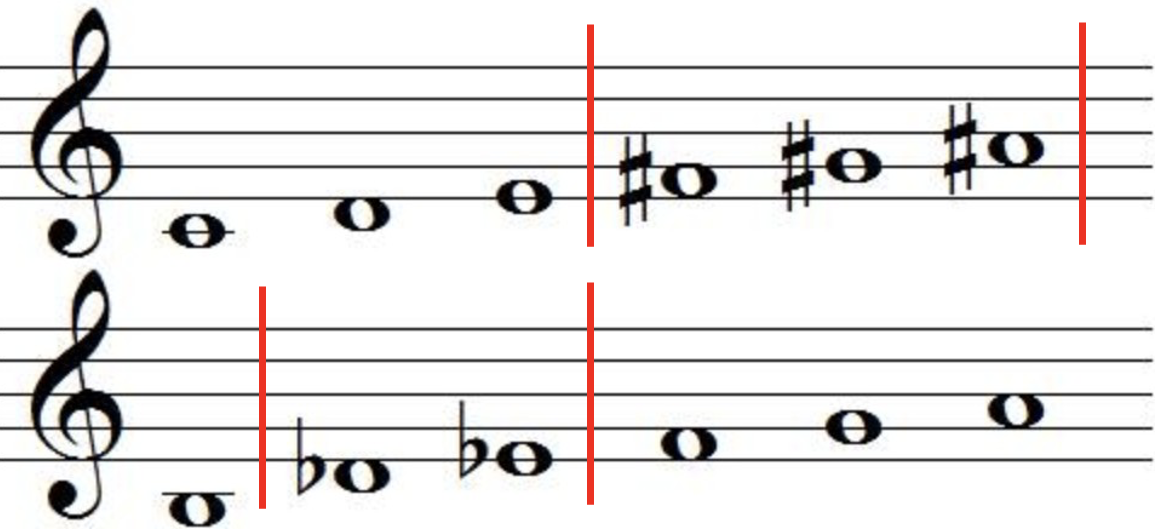
\includegraphics[width=0.25\textwidth]{images/whole_tone}
\caption{Whole Tone Scales}
\label{chromatic}
\vspace{-3mm}
\end{figure}

To determine the next note name, we thus simply traverse up or down the C major scale, excluding the appropriate ``skip" note. The accidental changes for both scales are bounded on one end by their respective ``skip" notes; the other ends are bounded by E in the ascending scale and F in the descending scale. To determine the next accidental, we thus appropriately lift or lower the current accidental at these boundaries, otherwise leaving it unchanged.

\subsubsection{Chords and Arpeggios}
\label{sec:chord_expansion}
Each note in the chord or arpeggio is generated with the logic from Section \ref{sec:note_generate} based on their respective intervals from the tonic (i.e. the chordal root). Chordal thirds, fifths, and sevenths have respective intervals of 2, 4, and 6 from the tonic. 

The imperfect chordal intervals are set to major for major and augmented chords, and minor for minor, half diminished, and fully diminished chords. Thus, for augmented chords, the chordal fifth accidental must be lifted, and the seventh must be lowered. For diminished chords, the  fifth and seventh must be lowered, and for half diminished chords, the  fifth  alone must be lowered.

To handle inversions, recall that the chord (whether triad or seventh) starts out in root position. Let $n$ be the desired inversion value (0 for root, 1 for first inversion, 2 for second,  and 3 or third). By incrementing the octaves of the first $n$ tones of the chord in root position, we obtain the correct inversion. 

If the chord is an arpeggio, we simply return a series of individual notes, rather than a simultaneous cluster.

\subsubsection{Cadences}
A cadence is expanded to the lists of chords it comprises. Thus, two levels of expansion occur here: an intermediate step from cadence to chord templates, and the final step from chord templates to notes.

Recall that the chords in each cadence are defined in Section \ref{table:cadences}, which reveal the interval of each chordal root from the tonic. Using this, for each chord in the cadence, we first employ the logic from Section \ref{sec:note_generate} to generate the root note of each chord. Then, we use the logic in Section \ref{sec:chord_generate} to generate a template for each chord, which undergo a second expansion in Section \ref{sec:chord_expansion}. 

The scale quality given to Section \ref{sec:chord_generate} to generate the chord template is generally that of the cadence. However, there are exceptions. All V chord templates are generated within a major scale, no matter the cadence quality, since cadences always have major V chords. Similarly, we want the seventh triad in the imperfect authentic cadence to be diminished  -- i.e. built on the major seventh -- no matter the local key quality (since we raise the leading tone in minor keys when moving towards the tonic), which means this chord template must also be generated within a major scale in Section \ref{sec:chord_generate}. 

The tonic octave supplied for the chord template generation in Section \ref{sec:chord_generate} is also usually that of the cadence. However, in order for the cadence to follow smooth voice leading, the tonic octave given for generating all second inversion triads, which appear in all cadences except perfect authentic, must be lowered once in relation to the specified cadence octave. This is demonstrated in the B major deceptive cadence in \figref{fig:cadence_octaves}. After converting to root position for clarity, notice how the chordal root in the cadence octave is in blue, and the roots an octave below (i.e. those of the second inversion triads) are in red.
\vspace{-2mm}
\begin{figure}[h!]
\centering
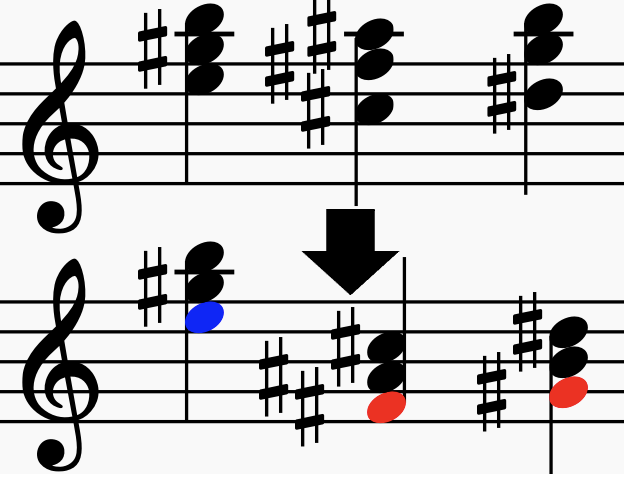
\includegraphics[width=0.18\textwidth]{images/cadence_octaves}
  \caption{Deceptive Cadence Octave Analysis}\label{fig:cadence_octaves}
\end{figure}
\vspace{-4mm}
\subsubsection{Harmonic Sequences}
Similar to cadences, harmonic sequences are initially expanded to the chord templates they comprise, which then undergo a second expansion to notes. Recall from \figref{table:harmseq} that each sequence consists of 14 chords, after which it cycles an octave above or below, depending on the direction of the sequence.

In order to generate chord templates for a sequence, we need to determine 
\vspace{-1mm}
\begin{enumerate}
\itemsep0em 
\item the interval between each pair of chordal roots, which dictates how to proceed from one chord to the next in the sequence
\item the inversion of the each chord
\item the octave number of each chord (given by the chordal root octave) relative to the tonic
\end{enumerate}

To determine (1) and (2), consider the analysis in \figref{fig:desc_56_intervals}, which determines the interval pattern for the chordal roots of the descending 5-6 sequence (as defined in \figref{table:harmseq}), given the zero-based sequence index of each chord. 

\begin{figure}[h!]
\centering
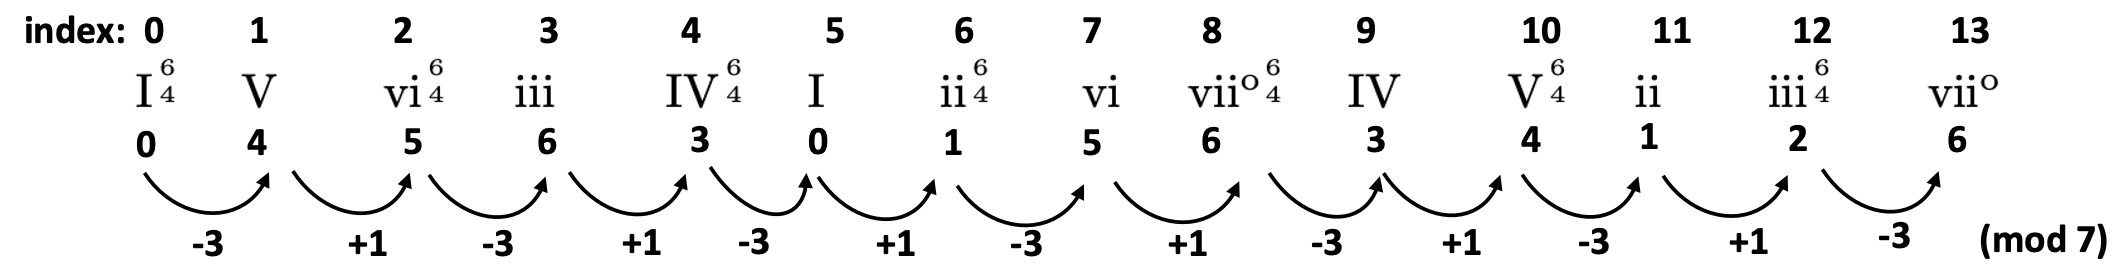
\includegraphics[width=0.5\textwidth]{images/desc_56_intervals}
  \caption{Descending 5-6 Interval Analysis}\label{fig:desc_56_intervals}
\end{figure}
\vspace{-3mm}
The top row is the chord index, the second row is the chord progression from \tabref{table:harmseq}, the third row is the interval between each chordal root and the tonic, and the bottom row is the interval between each chordal root and the previous (modulo 7). A clear pattern for inversions (in the second row) and interval changes (in the fourth row) emerges based on the parity of the index. Identical analyses are applied to the remaining sequences to formalize their interval and inversion patterns.

Finally, we need to determine (3), the octave number of each chordal root relative to the tonic, or the root of the first chord in the sequence. Consider \figref{fig:desc56-example}, which presents an octave analysis for the descending 5-6 sequence. 
\vspace{-2mm}
\begin{figure}[h!]
\centering
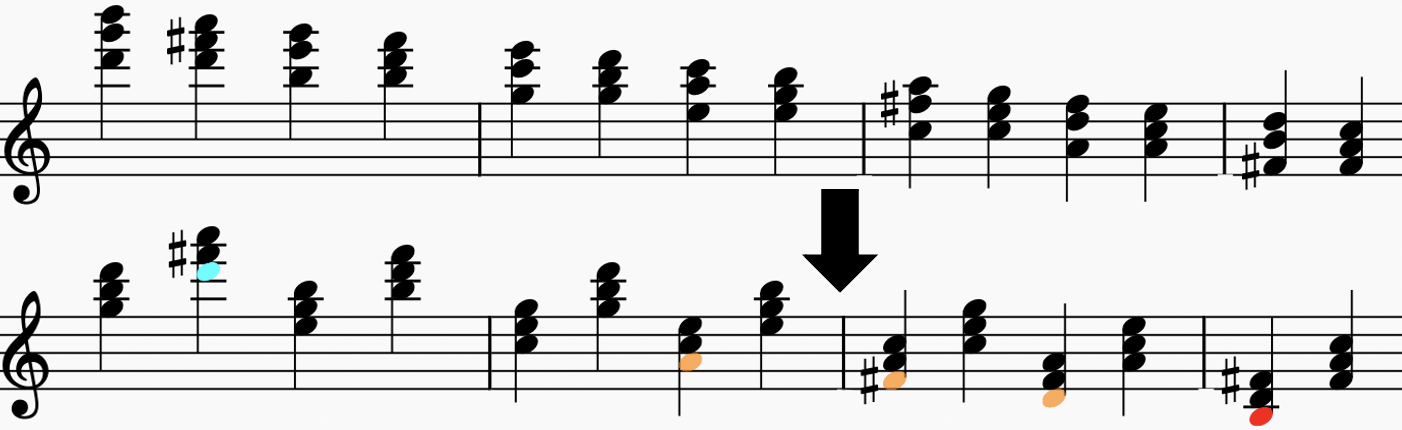
\includegraphics[width=0.45\textwidth]{images/desc56-example}
  \caption{Descending 5-6 Octave Analysis}
  \label{fig:desc56-example}
\end{figure}
\vspace{-3mm}

All chords are converted to root position in order to visualize the octave numbers of their roots in relation to the tonic. The chordal roots in blue are an octave number above the tonic, the roots in yellow are an octave below, and the root in red is two octaves below. This same analysis is applied to determine the octave numbers of the chords in the remaining sequences.

Importantly, the interval analysis in \figref{fig:desc_56_intervals} holds for any representation of a harmonic sequence, as this is what defines the musical theoretical structure. However, the inversion and octave analyses in Figures \ref{fig:desc_56_intervals} and \ref{fig:desc56-example} hold only for MusAssist's chosen representation of the sequences in \tabref{table:harmseq}, as a different inversion scheme would alter their outcomes.

%-----------------------------------------------------------------------------------------------------------------------------------------------------

\section{Conclusion}
This paper presents MusAssist, an external, declarative DSL for music notation that closes the abstraction gap between music theory and written composition. Users can uniquely write specifications in MusAssist's simple and high-level syntax for scales, chords, arpeggios, cadences, and harmonic sequences at the precisely levels of abstraction of the musical theoretical structures they describe. Fundamental musical elements such as notes, rests, custom note collections, new measures, and key signatures are also supported, along the ability to reuse labeled expressions and indicate comments. MusAssist programs are translated by its Haskell-based compiler to MusicXML so that the composition can be loaded into notation software for further manual editing. 


Optimally, in the future MusAssist would support templates for additional non-diatonic structures like octatonic and penatotic scales, as well as all flavors of suspended, ninth, eleventh, and thirteen chords (often seen in jazz). Templates for key modulations (i.e. specifications for generating a sequence of chords that successfully modulates from one key to another) are also planned. Furthermore, MusAssist would ideally increase the customizability of existing templates that are not fully expressive.  The current MusAssist template expansions for cadences and harmonic sequences are limited to the representation schemes outlined in Tables \ref{table:cadences} and \ref{table:harmseq}. In order for MusAssist to fully close the abstraction gap between the musical theoretical structures it formalizes and their low-level notational forms, all theoretical variations of the structures within the principles of functional harmony should be supported. Support for two-clef composition (as opposed to the current single-clef system) would allow for cadences and harmonic sequences, as well as future complex templates like key modulations, to better align with their musical theoretical definitions by including the essential baseline. Finally, user studies of MusAssist would give  insight into potential improvements for language design. 

\begin{acknowledgments}
I am very grateful to Professor Ben Wiedermann of Harvey Mudd College for his invaluable mentorship throughout this project.
\end{acknowledgments} 

%%%%%%%%%%%%%%%%%%%%%%%%%%%%%%%%%%%%%%%%%%%%%%%%%%%%%%%%%%%%%%%%%%%%%%%%%%%%%
%bibliography here
\bibliography{icmc2021template}

\end{document}
